\documentclass[IEEEtran,letterpaper,10pt,titlepage,draftclsnofoot,onecolumn]{article}

\usepackage{nopageno}
\usepackage{alltt}
\usepackage{float}
\usepackage{color}
\usepackage{url}
\usepackage{balance}
\usepackage{enumitem}
\usepackage{pstricks, pst-node}
\usepackage{geometry}
\geometry{textheight=9.5in, textwidth=7in}
\newcommand{\cred}[1]{{\color{red}#1}}
\newcommand{\cblue}[1]{{\color{blue}#1}}
\usepackage{hyperref}
\usepackage{textcomp}
\usepackage{listings}
\usepackage{graphicx}

\definecolor{dkgreen}{rgb}{0,0.6,0}
\definecolor{gray}{rgb}{0.5,0.5,0.5}
\definecolor{mauve}{rgb}{0.58,0,0.82}
\lstset{frame=tb,
  language=c,
  aboveskip=3mm,
  belowskip=3mm,
  showstringspaces=false,
  columns=flexible,
  basicstyle={\small\ttfamily},
  numbers=none,
  numberstyle=\tiny\color{gray},
  keywordstyle=\color{blue},
  commentstyle=\color{dkgreen},
  stringstyle=\color{mauve},
  breaklines=true,
  breakatwhitespace=true,
  tabsize=3
}

\def\name{Emily Longman, Zach Rogers, and Dominic Giacoppe}

\title{Requirements Document}
\author{Emily Longman, Zach Rogers, and Dominic Giacoppe}


\begin{document}
\begin{titlepage}
  \begin{center}
    \vspace*{1cm}

    \huge
    \textbf{Requirements Document}
  \vspace{0.5cm}

    \textit{Security for Robotics}\\
  \vspace{0.5cm}

    \textit{Emily Longman, Zach Rogers, and Dominic Giacoppe}\\
  \vspace{0.5cm}
    \vfill
    \large
    \textbf{CS461 Capstone}\\
  \vspace{5mm}
    \textbf{11/04/2016}\\

  \vspace{2in}
  \makebox[2.5in]{\hrulefill} \hspace {1.0in}\makebox[2.5in]{\hrulefill} \\
  Sponsor \makebox[2.5in][r]{Date} \\

  \vspace{.2in}
  \makebox[2.5in]{\hrulefill} \hspace {1.0in}\makebox[2.5in]{\hrulefill} \\
  Group Member \makebox[2.5in][r]{Date} \\

  \vspace{.2in}
  \makebox[2.5in]{\hrulefill} \hspace {1.0in}\makebox[2.5in]{\hrulefill} \\
  Group Member \makebox[2.5in][r]{Date} \\

  \vspace{.2in}
  \makebox[2.5in]{\hrulefill} \hspace {1.0in}\makebox[2.5in]{\hrulefill} \\
  Group Member \makebox[2.5in][r]{Date} \\

    \vfill
    \end{center}
\end{titlepage}

\subsection*{Introduction}

\subsubsection*{Purpose:}
To define the requirements and deliverables for (team name)'s capstone project to our sponsor, Vedanth Narayanan.

\subsubsection*{Scope:}
We are to find security vulnerabilities in ROS/SROS, document these vulnerabilities, and if possible, produce patches for anything we find. Any patches produced will be submitted to the ROS project. Our testing will be focused around ROS/SROS running on a drone, and we will see if we can compromise that drone based on our findings.

\subsubsection*{Definitions:}

\begin{itemize}
  \item Vulnerability: Any exploitable piece of code or system that would allow unauthorized users to interact with/damage/control the system, especially in a malicious manner.
  \item ROS: Robot Operating system, as found at link
  \item SROS: Secure ROS; a project based on ROS with the goal of implementing various security standards.
\end{itemize}

\subsection*{Overall}

\subsubsection*{Perspective:}
All software developed by (Team name) should have 2 objectives:
1. Fixing a specific, known vulnerability in ROS/SROS
2. Be lightweight enough that the implementation doesn't drastically affect the overall operation of the robot. Ideally, any code produced would be later incorporated into ROS itself, and not an external layer or program.

\subsubsection*{Software Interfaces:}
As we are looking for vulnerabilities in ROS, all code produced must be compatible with it or integrated into it. The version of ROS we will be using is TBD.

\subsubsection*{Communications Protocol:}
ROS uses 2 major forms of communication. Internally, ROS has the publisher subscriber system, which works basically like a socket system.
Publishers export data, and anyone who subscribes to that publisher receives the data, with no limit to the number of
subscribers or any authentication on who can subscribe. There is also normally some sort of wireless/wired connection to a base
station, which controls the starting and stopping of the robot. These generally take the form of a standard LAN connection,
although with extra effort more complicated setups are possible. (SOURCE)

\subsubsection*{Specific Requirements:}
As previously stated, at the moment (Team Name) is in the process of finding specific vulnerabilities. When we do find one, we will produce documentation outlining at least but not limited to:
Our operating environment, the type of attack, the particular system/piece of code attacked, the success rate of the attack, the result of the attack, and the potential fix to prevent the attack.


\subsubsection*{Gantt Chart:}
\begin{figure}
  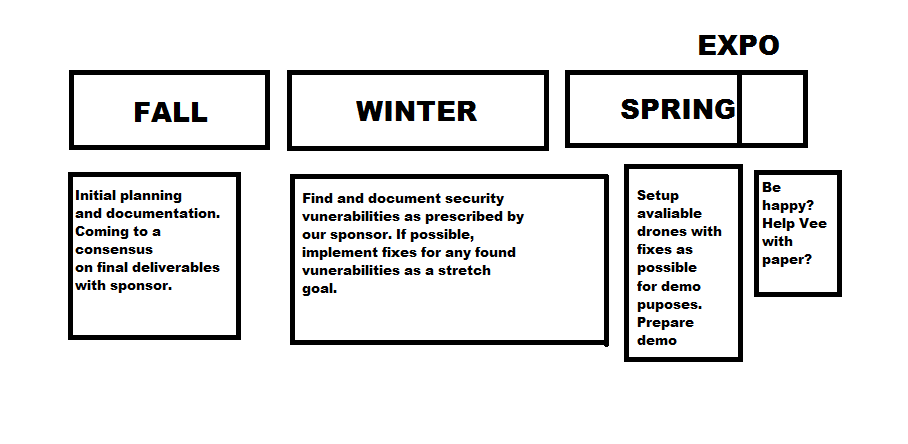
\includegraphics[width=\linewidth]{gantt.png}
  \caption{Gantt Chart}
  \label{fig:gantt}
\end{figure}

\clearpage

\nocite{*}
\bibliographystyle{IEEEtran}
\bibliography{ProblemStatement.bib}

\end{document}
